\documentclass[conference]{IEEEtran}
\IEEEoverridecommandlockouts
% The preceding line is only needed to identify funding in the first footnote. If that is unneeded, please comment it out.
\usepackage{cite}
\usepackage{amsmath,amssymb,amsfonts}
\usepackage{algorithmic}
\usepackage{graphicx}
\usepackage{textcomp}
\usepackage{xcolor}
\usepackage{footnote}
\usepackage{multicol}
\usepackage{float}
\usepackage{url}[hyphens]
\usepackage[acronym, nonumberlist]{glossaries}

\def\BibTeX{{\rm B\kern-.05em{\sc i\kern-.025em b}\kern-.08em
    T\kern-.1667em\lower.7ex\hbox{E}\kern-.125emX}}
\begin{document}

\title{On demand virtual Information Centric Networking (ICN) environment for sharing digital objects across different data infrastructures
}

\author{\IEEEauthorblockN{Kees de Jong, Cas Fahrenfort, Anas Younis, Zhiming Zhao}
\IEEEauthorblockA{\textit{System and engineering lab} \\
\textit{University of Amsterdam}\\
Amsterdam, the Netherlands \\
kees.dejong@surfsara.nl, casfahrenfort@live.nl, anas.younis@os3.nl, z.zhao@uva.nl}
}

\maketitle

\begin{abstract}
Data infrastructures manage the life cycle of data assets and allow users to efficiently discover and assess data. To improve its assets \gls{fairness}, a data infrastructure needs to provide data assets rich meta information, to describe its semantics contextual information and globally resolvable identifiers. The \glspl{pid}, like \gls{doi} are often used by data publishers and infrastructures. The traditional IP network approach and client-server model for data access can potentially cause congestion and delays with many data consumers. In contrast, the \gls{icn} such as \gls{ndn} adopts a data centric approach where digital data objects, once requested, may be stored on intermediate hops in the network. Consecutive requests for that unique digital object are then made available by these intermediate hops (caching). This approach distributes traffic load more efficient and reliable compared to host-to-host connection oriented techniques, and demonstrates attractive opportunities for sharing digital objects across distributed networks. However, such an approach also faces several challenges. It requires not only an effective translation between the different naming schemas among \gls{pid} and \gls{ndn}, in particular for supporting \gls{pid} from different publishers or repositories. Moreover, the planning and configuration of an \gls{icn} environment for distributed infrastructures are lacking an automated solution. To bridge the gap, we propose an \gls{icn} planning service with specific consideration of interoperability across \gls{pid} schemas in the Cloud environment.
%Data infrastructures manage data across their lifecycle, and provide them  of massive data, and provide them, this data is published by the use of \glspl{pid}. The traditional network approach for data transmissions are done with host-to-host connections (IP), where every data request from the consumer is answered with a data transfer from the source (the producer). This approach can potentially cause congestion and delays with many data consumers. \gls{ndn} is a data centric approach where unique data, once requested, may be stored on intermediate hops in the network. Consecutive requests for that unique digital object are then made available by these intermediate hops (caching). This approach distributes traffic load more efficient and reliable compared to host-to-host connection oriented techniques.

%The \glspl{pid} are used by data providers within these data infrastructures for sharing and identifying digital objects. In order to create \gls{pid} and \gls{ndn} integration, a translation between the different naming schemas is needed. This paper proposes a solution for accessing and sharing digital objects with different \gls{pid} schemas over a networked environment using \gls{doip} and \gls{ndn}. Furthermore, a solution is proposed to plan and deploy an \gls{ndn} with a scalable method for Cloud environments.
\end{abstract}

\begin{IEEEkeywords}
Named Data Networking, Persistent Identifier, Digital Object Interface Protocol, FAIRness, Network Functions Virtualization
\end{IEEEkeywords}

\section{Introduction}
Data infrastructures manage the life cycle of data assets, and allow users to effectively discover and utilize data for their specific purposes. Typical examples include EuroArgo\footnote{\url{https://www.euro-argo.eu/}} and SeaDataNet\footnote{\url{https://www.seadatanet.org/}} for ocean observation data, \gls{icos} \footnote{\url{https://www.icos-ri.eu/}} and \gls{actris}\footnote{\url{https://www.actris.eu/}} for air monitoring data, and \gls{epos}\footnote{\url{https://www.epos-ip.org/}} for solid earth monitoring. Those data infrastructures (sometimes also called research infrastructures) become important facilities for enabling data centric research, and can significantly enhance the feasibility for research at the system level, e.g., for studying global climate change and natural disasters.

However, to effectively discover and utilize resources across different infrastructures, users still face the challenges of limited \gls{fairness} of digital assets. It becomes a common problem for many research infrastructures to improve their \gls{fairness}; several projects have been funded for this purpose. The EU recently funded project ENVRI-FAIR\footnote{www.envri-fair.eu} is a such effort for improving the \gls{fairness} for more than 10 environmental research infrastructures. In this context, the globally resolvable identifier (also called (\gls{pid})) of digital objects and their rich contextual metadata are often highlighted as important aspects, as recommended in the 11 principles of \gls{fairness}\footnote{\url{https://www.force11.org/}}.

Moreover, the classical client-server or P2P solutions are lacking support for distributing digital objects from heterogeneous repositories, in particular for handling continuously growing data quantity, sources and involved users. Protocols like the \gls{doip} have also been recommended by the community of \gls{rda} to handle the sharing of digital objects. However, it is still challenging to share data with \glspl{pid} among the different infrastructures.

%However, to effectively discover and utilise resources across different infrastructures, users still have to face the challenges of limited \gls{fairness} of digital assets. Many research infrastructures face the common challenge to improve their \gls{fairness}. The EU recent funded project ENVRI-FAIR \footnote{www.envri-fair.eu} is such an effort for improving the \gls{fairness} for more than 10 environmental research infrastructures. In this context, the globally resolvable identifier (also called (\gls{pid})) of digital objects and their rich contextual metadata are often highlighted as important aspects, as recommended in the 11 principle of \gls{fairness} \cite{}. Some research infrastructures have already adopted \gls{doi} or other types of \gls{pid} solutions for publishing their digital objects, e.g., in \gls{icos}.

%In many scientific domains, massive data collected from observations, simulations and system logs, become important assets for enabling further data centric sciences e.g., modelling complex environment problem requires a long history of observation data \cite{}. After careful curation, data become an important asset in data infrastructures. Typical examples include ocean observation data in EuroArgo\footnote{\url{https://www.euro-argo.eu/}} and SeaDataNet\footnote{\url{https://www.seadatanet.org/}}, air monitoring data in the \gls{icos} research infrastructure\footnote{\url{https://www.icos-ri.eu/}} and \gls{actris}\footnote{\url{https://www.actris.eu/}}, and solid earth monitoring in \gls{epos}\footnote{\url{https://www.epos-ip.org/}}. Those continuously growing data from different research infrastructures provide valuable input from different domains, and can significantly enhance the feasibility for doing research at the system level, e.g., for studying climate change and natural disasters. However, users still have to face several challenges to effectively discover and utilise those assets.

%The limited \gls{fairness} of digital assets prevents users from effectively discovering digital assets from distributed sources and obtaining their content for specific purposes. It becomes a common challenge for many research infrastructures to improve \gls{fairness}; \gls{envri} is such an effort, recently funded for improving the \gls{fairness} for more than 10 environmental research infrastructures. The globally resolvable identifier (also called (\gls{pid})) of digital objects and their rich contextual metadata are often highlighted as important aspects when improving the \gls{fairness}, as recommended in the 11 principle of \gls{fairness} \cite{}. There are already quite some research infrastructures that have already adopted \gls{doi} or other types of \gls{pid} solutions for publishing their digital objects, e.g., in \gls{icos}.

%Moreover, the classical client-server or P2P solutions for sharing and distributing digital objects has to face the challenges of heterogeneous repositories cross infrastructures, diverse granularity of digital objects, and continuously growing scale of the data quantity, sources and involved users. The \gls{eosc} is moving towards the direction of providing an open ecosystems for different parties to effectively share their services and data, and to utilise them in the life cycle of their research activities. Protocols like the \gls{doip} have also been recommended by the community of \gls{rda} to handle the sharing of digital objects. However, it is still challenging to share data with heterogeneous sizes and \glspl{pid} among the different infrastructure.

On the other hand, the networking technologies have made significant progress during the past years for improving the distribution efficiency, e.g., \gls{icn} \cite{zhang2014named}, for application aware adaptability, e.g., \gls{sdn} \cite{kreutz2014software}, and for effectively resource management and sharing over common network infrastructures, e.g., \gls{nfv} \cite{han2015network}. Those advanced technologies still lack seamless support for being embedded in the data management life cycle, e.g., for discovering and sharing digital objects with \glspl{pid}. In the earlier papers \cite{koulouzis2018information}, Koulouzis et al. discussed the feasibility to use \gls{icn} solutions like \gls{ndn} to distribute the digital objects with \glspl{pid}; however, the work only focused on the \glspl{pid} from a single publisher. Cloud caching \cite{dash_economic_2009} and data lake \cite{6949519} are other types of solutions which focus on smart caching of the digital objects across distributed infrastructures, but did not have an explicit model of the data contents global resolvable identifiers.

In this paper, we extend our earlier work of \gls{naas4pid} \cite{koulouzis2018information}, and specifically look at three aspects in applying \gls{ndn} in data infrastructures: 1) how to seamlessly publish version controlled digital objects with \gls{pid}, 2) how to plan and deploy a customized virtual \gls{ndn} environment for user communities on different infrastructures, and 3) how to distribute digital objects from distributed data sources with heterogeneous \gls{pid} publishers. We will use a case study from the SeaDataNet and structure the paper in five parts. First we will briefly introduce the pilot use case, and review the state of the art and related work. And then we will present the proposed solution and demonstrate its usage via the use case.



%This paper is divided into two parts. Section \ref{pid-interoperability} explores solutions to translate \glspl{pid} into \gls{ndn} compatible names. And section \ref{ndn-planning-deployment} explores solution to plan and deploy \gls{ndn} with scalability in mind.

\section{Problem background, challenges and related work}
\label{problem-background}
A data infrastructure often aggregates several data sources, and provide their metadata via catalogues for users to precisely discover data assets. A typical example of SeaDataNet is shown in Fig. \ref{fig:sdc_cur}. 
\begin{figure}[H]
\centering
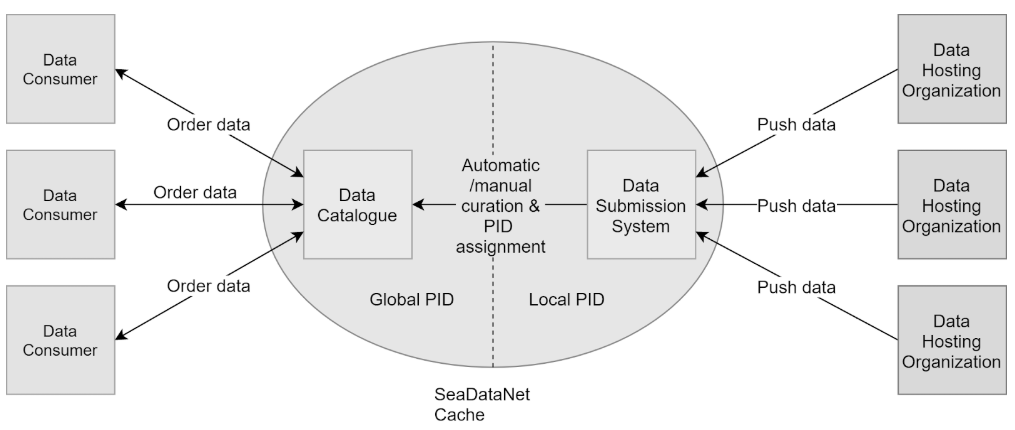
\includegraphics[width=\columnwidth]{images/SDC_current.png}
\caption{SeaDataNet's current infrastructure.}
\label{fig:sdc_cur}
\end{figure}
\subsection{Background}


To deliver high quality services to the user community, an infrastructure like the SeaDataNet often has to face several challenges:
\begin{enumerate}
    \item Fault tolerance challenges. The SeaDataNet originally only gathers metadata from remote repositories, and the user has to access the individual remote repository to obtain data. Such client-server style not only creates high load for the repository but also network traffic congestion.
    \item Performance challenges. A Cloud replica has been created in SeaDataNet to duplicate each remote repository in the Cloud. In this way, the clients can directly retrieve the copy of data assets from the Cloud server. However, such solution also needs careful customization for load-balancing and service placement to reach the required quality of service quality or user experiences.
    \item Scalability challenges. The SeaDataCloud has to face the continuous growth of both data providers and the user communities. In many cases, geo special data retrieval needs calculation of the region, layers and the time duration. The system has to face scalability challenges of both network and the server capacity. 
\end{enumerate}
In the rest of the section, we will review the related work of these topics and discuss the key contributions of our work. 

\subsection{Persistent Identifiers}
\label{sec:pids}

\glspl{pid} are in essence a permanent reference to a document, file, web page or data object. Generally, a \gls{pid} is assigned to a digital data object on request of the client, after which the service guarantees that whenever this identifier is resolved, it will provide necessary meta information about the digital object. \glspl{pid} do not guarantee that the digital object will be available forever; a \gls{pid} should still be resolvable (to the metadata) even if the digital object has been deleted. 

\glspl{pid} often have different `namespaces' which can be used to point to different sub-resolvers, much like how \glspl{url} can have different sub-domains. These namespaces can be used to allow a single resolver to resolve multiple top-level \glspl{pid} to a number of distinct resolvers which have their own \gls{pid} resolution system and separate repositories for storing data. This structure allows multiple different organizations to resolve data using a single \gls{pid} scheme, as long as they agree to uphold the persistence policies set by the top-level resolver. Typical schemas of \gls{pid} include \gls{doi}, \gls{urn} and \gls{purl}. \glspl{pid} are often provided by the third party registers, like the \gls{epic}, DataCite, ORCID, ISNI. 

%Cordra \cite{cordra} is an open-source Digital Object Management application, a core part of the \gls{doa} \cite{sharp2016overview}. It offers functionality for creating, editing and accessing digital objects as discrete data structures with unique, resolvable identifiers. Metadata is automatically extracted from any digital information (documents, images, spreadsheet data etc.) included in the objects and users may generate additional metadata themselves.

\subsection{\gls{pid} objects over ICN}
Karakannas proposed a mapping architecture for resolving \glspl{pid} to \gls{icn} names, and  for delivering big data with \glspl{pid} \cite{icn-bd}. This approach maps \gls{pid} to \gls{ndn} for every \gls{pid} type instead of implementing the translation on the clients browser.

Mousa researched the fetching and sharing of \gls{doi} objects with \gls{icn} such as \gls{ndn}. The researcher's approach focused only on \gls{doi} digital objects within \glspl{ndn}. The researcher explained that the difference in \gls{ndn} naming of different \gls{pid} providers must be taken into account, such that the correct prefix is used within \gls{ndn} to identify specific \gls{pid} types. In the researcher's design, the translation happens in the consumers' browsers. The consumer has the choice to either request the digital object by its \gls{ndn} name or \gls{pid} \cite{ndn-app-aware}.

Kolouzis et al. continued the research done by Karakannas \cite{icn-bd} and Mousa \cite{ndn-app-aware} and proposed an architecture to map \glspl{pid} into the naming schema of \gls{ndn}. A \gls{pid}2\gls{ndn} gateway was proposed for resolving \glspl{pid} to \gls{ndn} names, an \gls{ndn} node that implements a virtualized \gls{ndn} router, and an \gls{ndn}4\gls{pid} manager for automating the management of the \gls{ndn} overlay in Cloud or e-infrastructure.

\subsection{Named Data Networking}
\gls{ndn} is a popular ICN implementation, although it is not yet implemented on a large scale. There have been several large testbeds established during the past years, e.g., for scientific research in delivering climate data \cite{lim2018ndn}, and the hadron collider network \cite{shannigrahi2015named}. From those practices, \gls{ndn} provided performance improvements compared to classical climate data delivery techniques based on IP. In those work, cache size plays an important role in optimising performance, and a 1GB \gls{ndn} cache at the edge of the \gls{ndn} can already significantly improve data distribution and reduce the network load. However, native \gls{ndn} congestion control is still an open research area \cite{ren2016congestion}.
 
Koulouzis et al. investigated different strategies for caching, replacement and forwarding for different size data objects, and concluded that the `leave copy everywhere' caching strategy provided the best performance ratio between cache size to digital object size for generic data usage \cite{koulouzis2018information}. However, `leave copy down' and `leaving copies with probability' performed best for delivering big data objects. Koulouzis et al. also concluded that the ascending ordering of digital objects enhances network performance when combined with the `least recently used' caching strategy. Yuan et al. \cite{yuan2012scalable} used the \gls{ccnx} application\footnote{\url{https://wiki.fd.io/view/Cicn}} to investigate \gls{ndn} forwarding strategies, and concluded that packets with long names often degraded performance. Tortelli et al. researched the effectiveness of two opposite forward strategies; flooding and best-route (with and without caching) \cite{tortelli2013performance}. Several experiments lead them to the conclusion that there are pros and cons in each forwarding strategy. But that it is difficult to determine the best performing forward strategy. 
%After profiling the software they measured that the \gls{ndn} name decode operation took 35.46\% of the entire program running time. So et al. developed a method to achieve fixed lookup times with variable length names \cite{so2013named}. In order to achieve this goal they explored the application of hash tables to do name lookup. Furthermore, they explored the possibility to do this in hardware by using a Cisco ASR9000 router with the integrated service module running 64-bit Linux. With their experiments they managed to forward 20Gbps of real \gls{ndn} traffic. Tortelli et al. researched the effectiveness of two opposite forward strategies; flooding and best-route (with and without caching) \cite{tortelli2013performance}. Several experiments lead them to the conclusion that there are pros and cons in each forwarding strategy. But that it is difficult to determine the best performing forward strategy.
%This was concluded based on observations that if large digital objects were requested first, the cache replacement algorithm would make room by overwriting files already in the cache, resulting in cache misses. When small files were requested first, more cache hits were measured. As for cache size, the researchers recommended a cache size at least twice the size of the biggest digital object in the network \cite{koulouzis2018information}.

%Yuan et al. researched the performance of \gls{ndn} forwarding \cite{yuan2012scalable}. They used the \gls{ccnx} application\footnote{\url{https://wiki.fd.io/view/Cicn}} to perform experiments. Their research concluded that packets with long names degraded performance. After profiling the software they measured that the \gls{ndn} name decode operation took 35.46\% of the entire program running time. So et al. developed a method to achieve fixed lookup times with variable length names \cite{so2013named}. In order to achieve this goal they explored the application of hash tables to do name lookup. Furthermore, they explored the possibility to do this in hardware by using a Cisco ASR9000 router with the integrated service module running 64-bit Linux. With their experiments they managed to forward 20Gbps of real \gls{ndn} traffic. Tortelli et al. researched the effectiveness of two opposite forward strategies; flooding and best-route (with and without caching) \cite{tortelli2013performance}. Several experiments lead them to the conclusion that there are pros and cons in each forwarding strategy. But that it is difficult to determine the best performing forward strategy.


%Research Clouds such as proposed in the \gls{eosc} will offer Europe's 1.7 million researchers and 70 million science and technology professionals the means to store, share and re-use large volumes of information generated by the big data revolution. Research Clouds publish datasets from distributed sources, identified by a \gls{pid}. These datasets are not accessed via e.g. a simple web portal like traditional internet digital objects on the web. Instead these requests are processed by e.g. a data catalog of the federated research Cloud. Therefore, research Clouds face the challenge of identifying distributed data in a federated Cloud, provide data provenance and provide a scalable service to serve many users that request large datasets.

% This part is already discussed in the new introduction part by Zhiming
% Furthermore, research Clouds face a trend of increased data production and consumption, which is expected to grow. This general trend in research Clouds calls for a data distribution solution that better supports the scale and complexity. An example of such a research Cloud is SeaDataNet, which is a distributed marine data infrastructure network for managing the large and diverse data sets collected by the oceanographic fleets and the automatic observation systems. Their aim is to advance and increase the usage of SeaDataNet's services by adopting Cloud and high performance computing technology for better performance.

%Introducing the architecture in figure \ref{fig:sdc_cur} into an NDN is not solved yet. Multiple data providers need to be hosted, which potentially use different \gls{pid} schemas. \gls{naas4pid} is an extension of \gls{ndn} which allows it to interoperate with \glspl{pid} and is used by SeaDataNet. \gls{naas4pid} adds an additional system layer which translates \glspl{pid} to \gls{ndn} names and optimizes and manages the virtual \gls{ndn} overlay in Cloud or other e-infrastructures. However, \gls{naas4pid} currently only supports a single \gls{pid} provider.

Those practices and performance characteristics provide valuable information for designing and customising an \gls{ndn} environment.  

\subsection{Network planning and customization}
Planning and customizing the topology and capacity of a network is crucial to meet the requirements of applications. McCabe applies a systems methodology approach towards network design \cite{mccabe2010network}, and identifies three core phases (Fig. \ref{fig:mccabe-process}); analysis, architecture and design. These simple, yet important planning phases describe how to make technology and topology decisions in a network, especially for large deployments. 
%These decisions are guided based on inputs for these three core phases, the initial input may be from users and/or from network metrics. Consecutive processes use the output of previous processes as input, thus these processes are interconnected.

\begin{figure}[H]
\centering
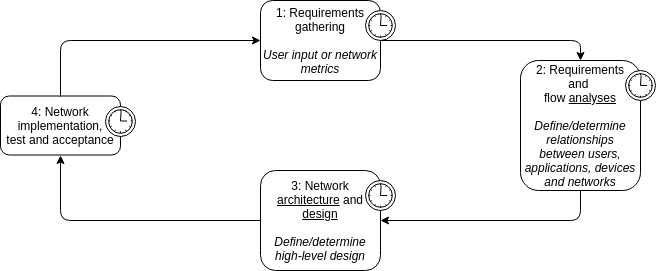
\includegraphics[width=\columnwidth]{images/mccabe-process.png}
\caption{Cyclic and iterative nature of McCabe's processes and phases.}
\label{fig:mccabe-process}
\end{figure}

Using the \gls{sdn} and other programmable network technologies, developers can control the flows via the service interface provided by the network control plane\cite{koulouzis_sdn-aware_2016}. Using the cloud environment, the virtual networks can be fully customized and manipulated based on the application constraints. In \cite{wang_planning_2017}\cite{wang_qos-aware_2017}, Wang et al., proposed a critical path based approach to plan a virtual infrastructure, including virtual machines, their topology, and the placement of \gls{sdn} controllers. Most of these work were so far mainly for the traditional IP based network. The planning solution for the \gls{icn} network is still quite limited. 



\subsection{Summary}
From the discussion, we can clearly see the advantages of using \gls{icn} technologies in distributing digital objects; however, the \gls{icn} has not yet been widely deployed as physical infrastructure, except experimental test beds. The \glspl{pid} of digital objects are crucial to make digital assets FAIR. However, not all data infrastructures are ready to provide their digital assets with \glspl{pid}. The \gls{pid} provides a natural mapping with the \gls{icn} solutions like \gls{ndn}; however, the seamless integration between \gls{ndn} and the heterogeneous \gls{pid} repositories are still a challenge.

In this context, we specifically highlighted three challenges in setting up \gls{icn} environments in Cloud: i) complexity of the data publishing and \gls{pid} assignment, ii) automation of virtual \gls{ndn} environment planning and provisioning and iii) interoperability among different \gls{pid} schema. 
To tack those challenges, we will bring the follow three contributions:
\begin{enumerate}
    \item Provide services to enable data managers to seamless publish data objects and obtain \glspl{pid} during the data management life cycle;
    \item Provide a network planner to plan virtual \gls{ndn} environments based on the characteristics of the data sources and user access patterns.
    \item Develop a \gls{pid} interoperability service in the \gls{ndn} for handling different \gls{pid} schema. 
\end{enumerate}

% From the discussion, we can clearly see the advantages of using ICN technologies in distributing digital objects; however, the ICN has not yet been widely deployed as physical infrastructure, except experiemntal test beds. The persistent identifiers of digital objects are crucial to make digital assets FAIR. However, not all data infrastructures are ready to provide their digital assets with PIDs. It is not only and provide a natural mapping with the ICN solutions like Named Data Networking; however, the seamless integration between NDN and the heterogeneous PID repositories is still a challenge. 
 

\section{Proposed solution}
An \emph{on demand \gls{ndn} environment manager for data infrastructures, or \gls{ndn4di}}, is proposed to facilitate the application of \gls{ndn} in the context of data infrastructure. Fig. \ref{fig:architecture-new} shows the basic idea. The system aims to provide support for 1) data manager to publish data objects and obtain the \gls{pid} for them, and 2) plan a customized \gls{ndn} environment in Clouds, and 3) automate the provision and deployment of the planned environment. After the \gls{ndn} environment is in operation, the \gls{ndn4di} also provides functions for handling \gls{pid} repositories from different publishers.  

\begin{figure}[ht]
\centering
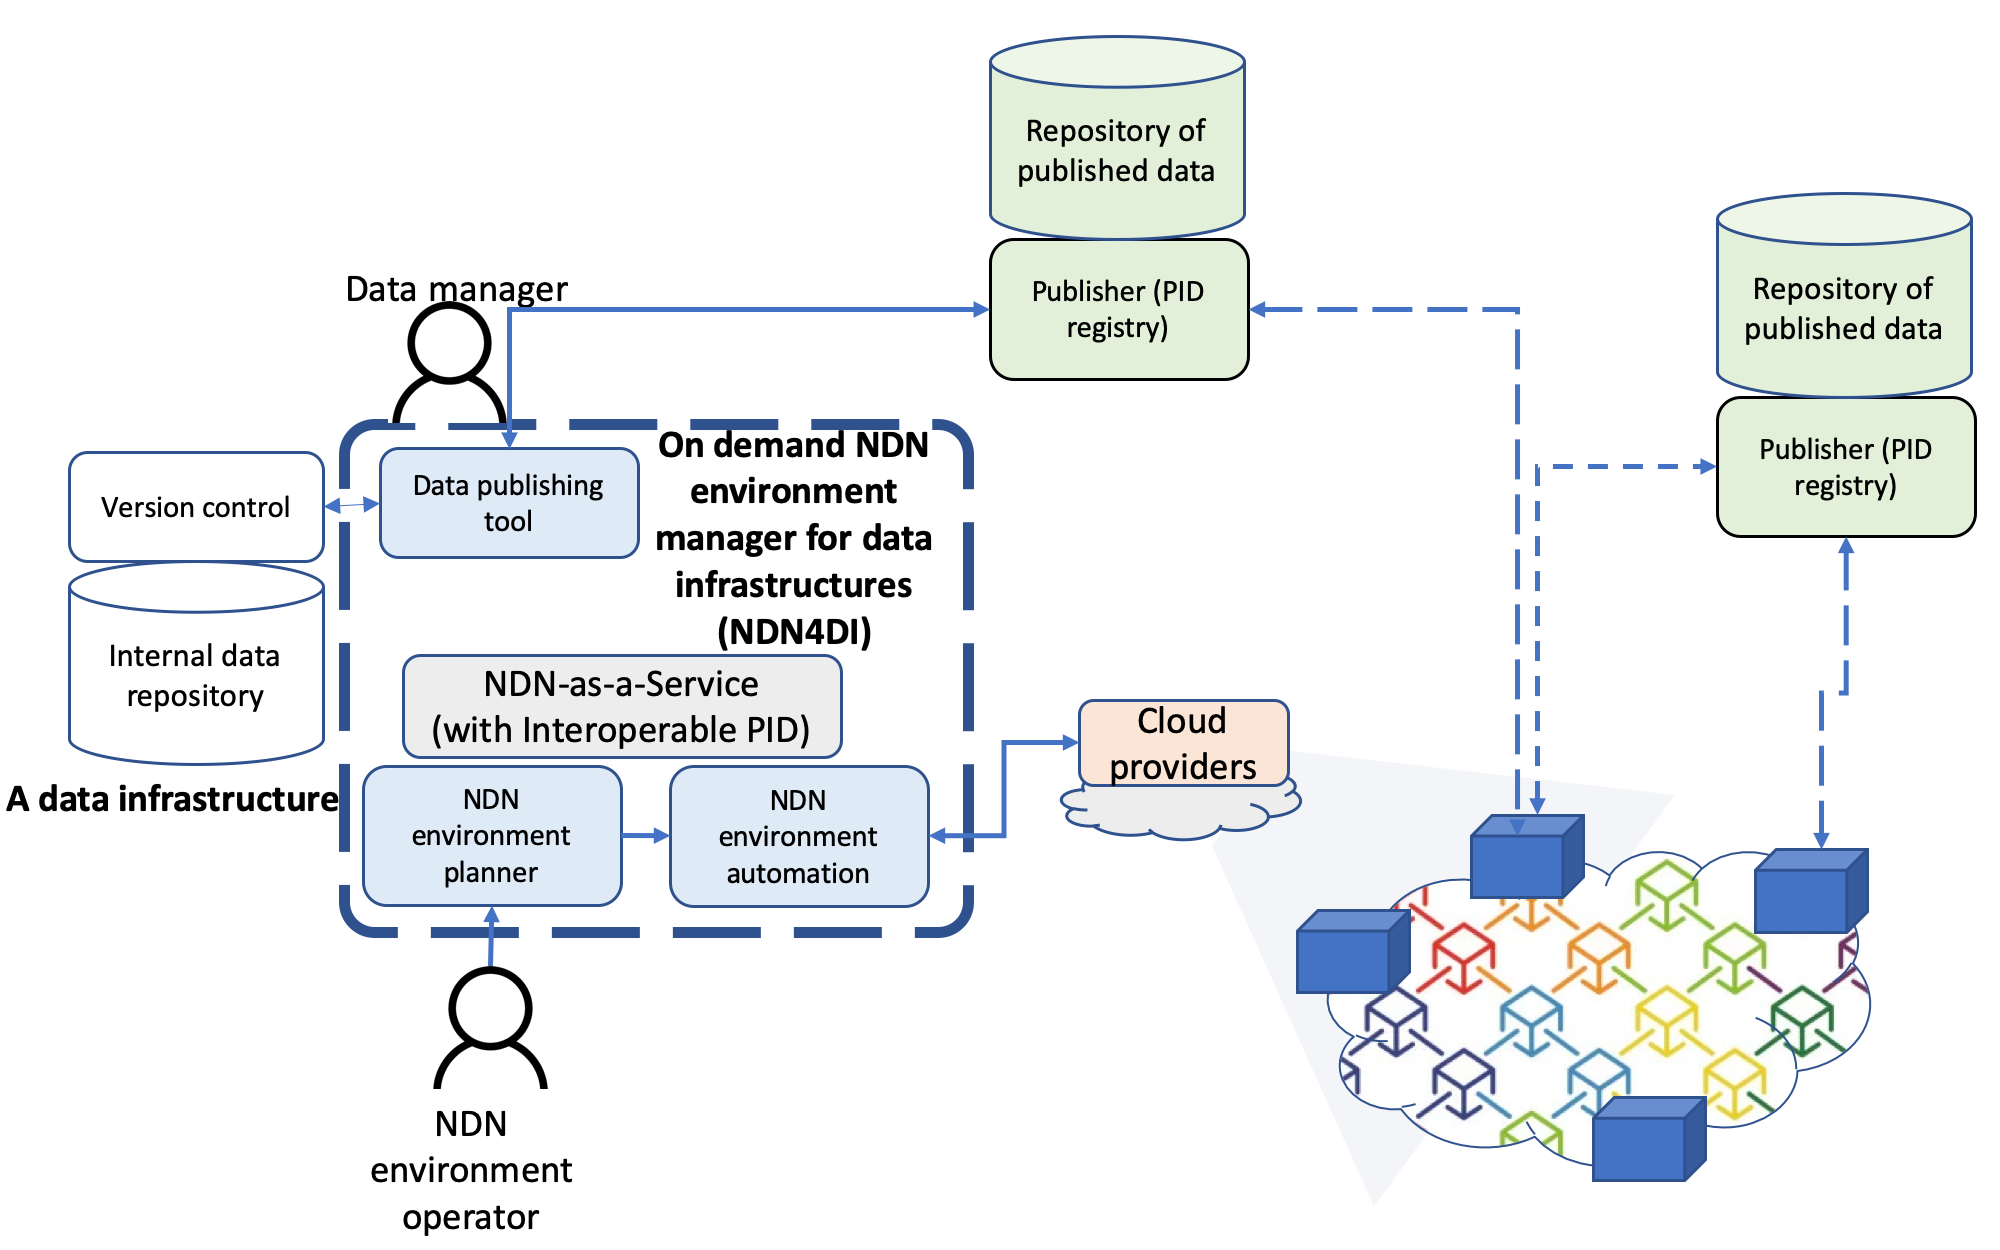
\includegraphics[width=\columnwidth]{images/NDN-pub-planner.png}
\caption{Basic idea of the proposed on demand \gls{ndn} planner solution for data infrastructures}
\label{fig:architecture-new}
\end{figure}

%\gls{fairness} is crucial for enabling open science and innovation based on digital objects (\glspl{pid}) from large communities of providers and users. However, the gaps among version control, identification and distributed access systems often make the scalability of data centric applications difficult across large user communities and highly distributed infrastructures. This section proposes a solution for accessing and sharing digital objects over a networked environment using \gls{doip} and \gls{ndn} by the use of \gls{naas4pid}. Furthermore, a \gls{pid} to \gls{ndn} translation prototype will be discussed with extensible support for \gls{pid} types in mind.


%\subsection{Technical considerations}
%\section{PID and NDN interoperability with version control}
%\label{pid-interoperability}

\subsection{PID assignment during data management}
Lots of existing data infrastructures are originated from early legacy systems, e.g., environmental observation stations, and lack of a global data identifier centered design for data services. The basic scenario is shown in the Fig. \ref{ndn-planning-deployment}. 

Following from the workflow in Fig. \ref{fig:sequence}, it is divided into three distinct parts: version control system, data publication and data distribution. Content created by community content providers is processed and stored (in its internal repository) by the version control system in any form that is required by its specific use case. Once submitted content has been approved, it is published to persistent data and metadata repositories by any \gls{pid} system. From there, the data can be discovered and accessed by content consumers through the \gls{ndn} by the use of the \gls{naas4pid} service.

\begin{figure}[ht]
\centering
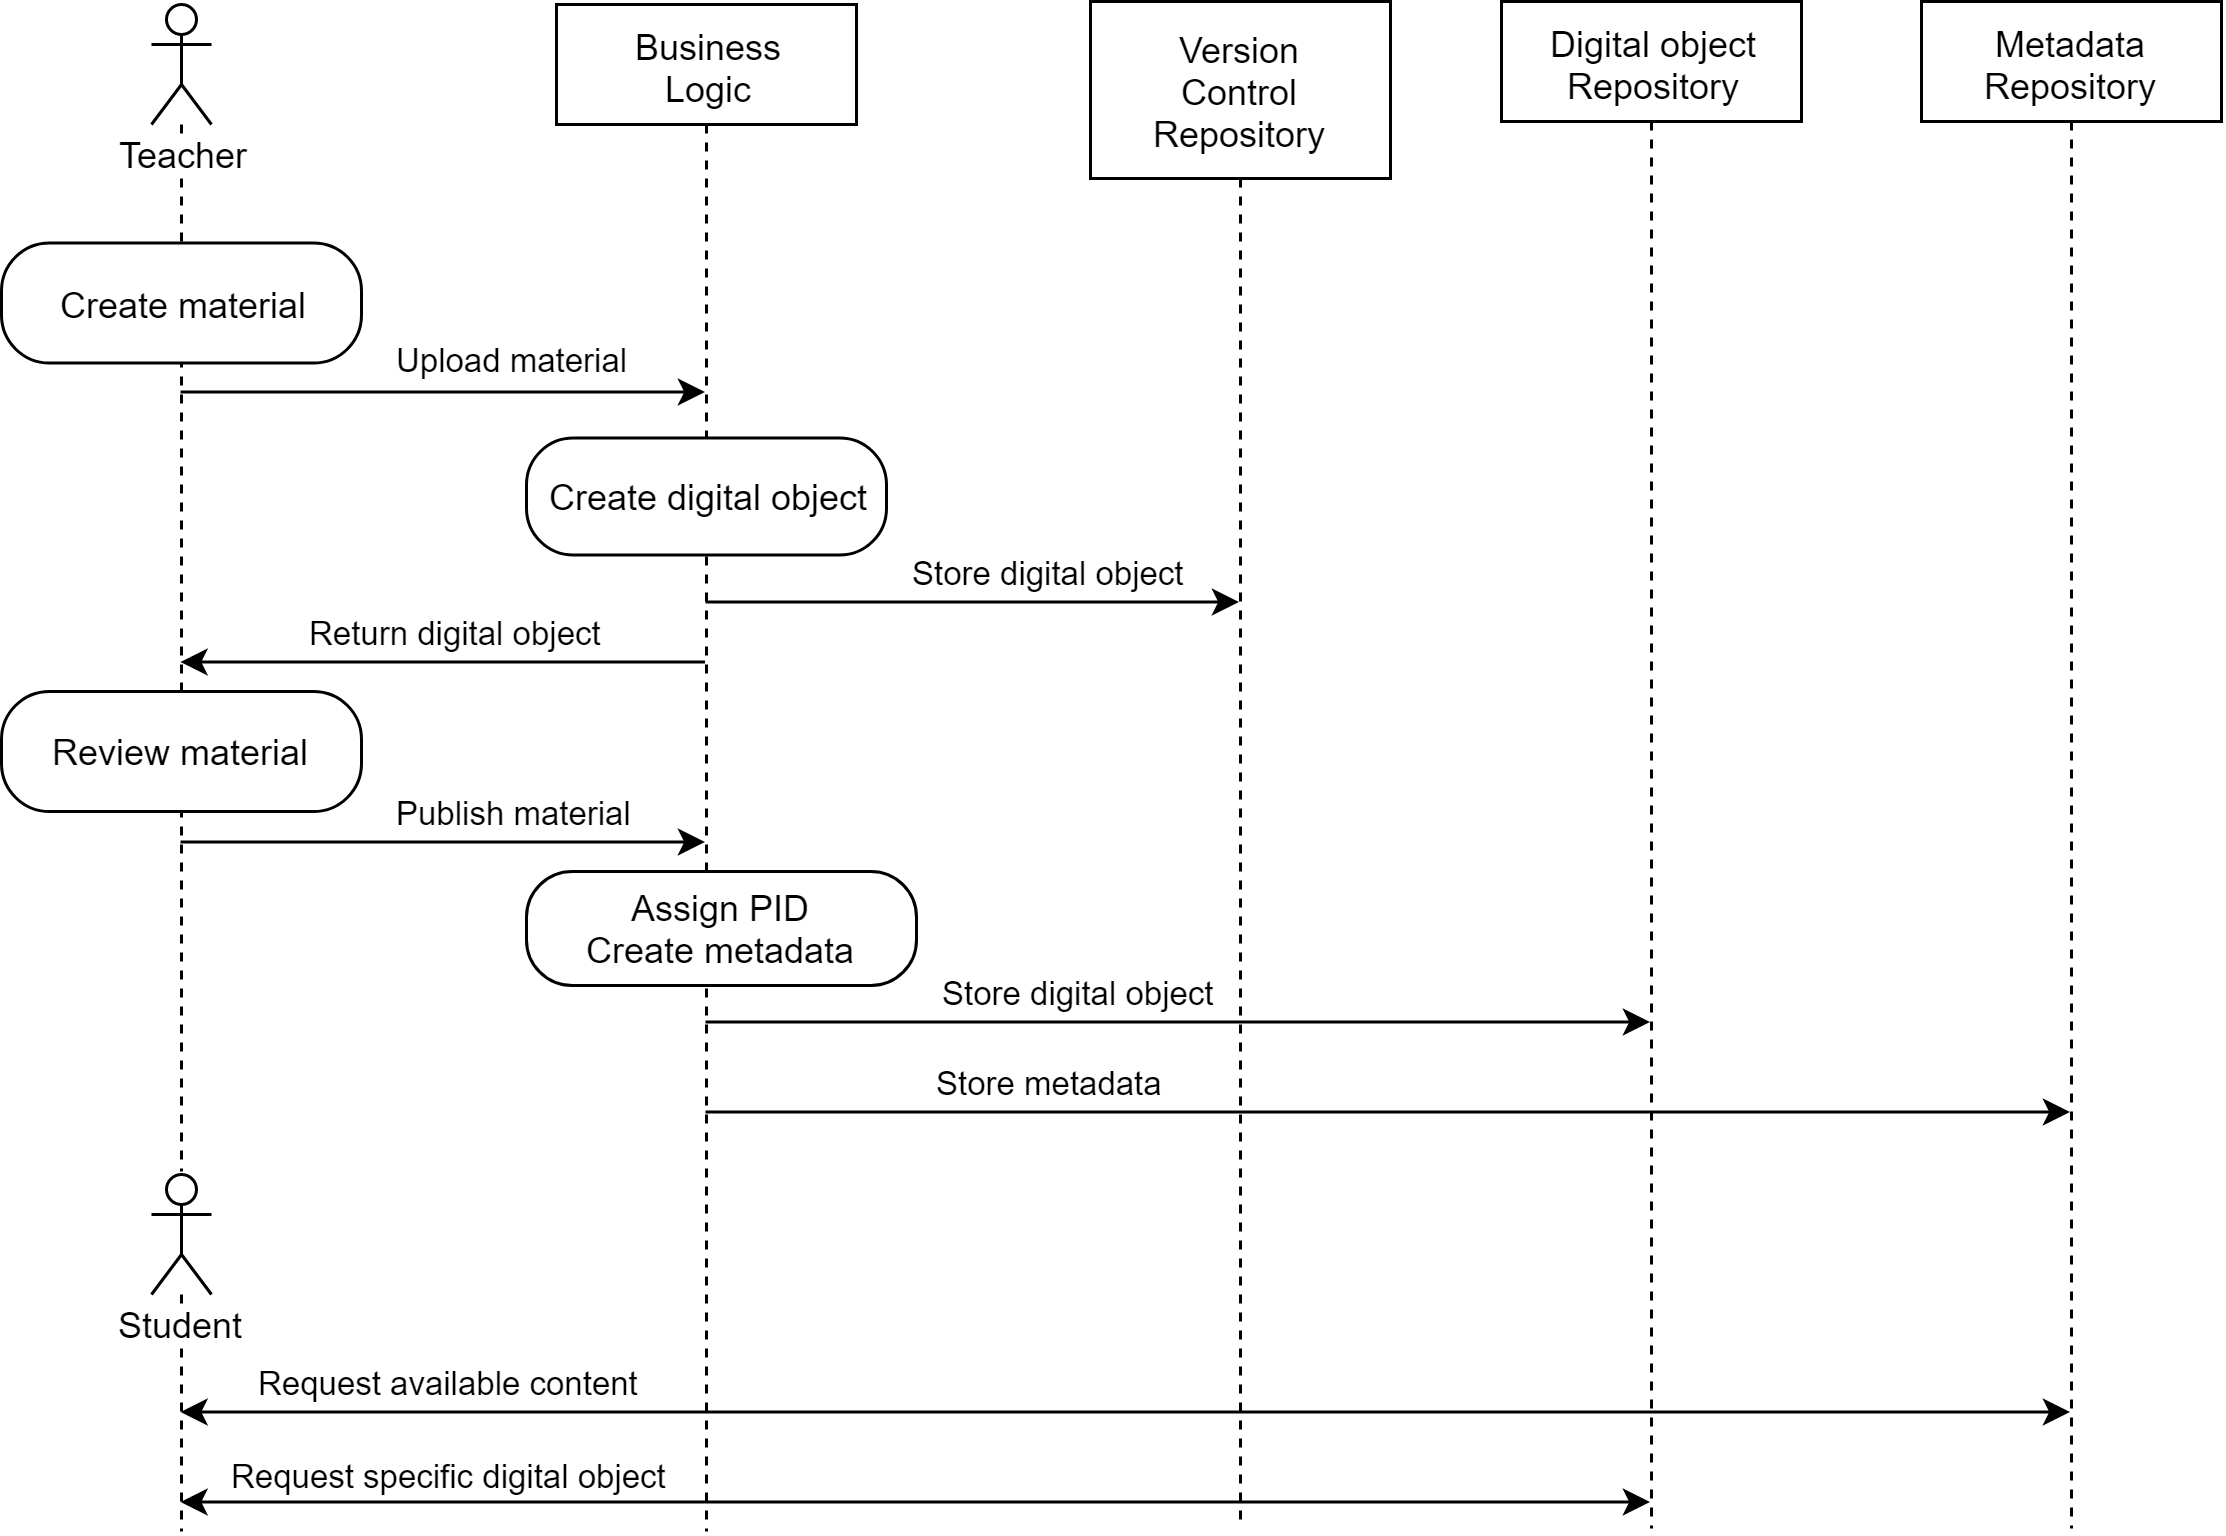
\includegraphics[width=0.4\textwidth]{images/sequence.png}
\caption{A basic scenario for publishing data objects from a version control system. }
\label{fig:sequence}
\end{figure}


\subsection{Support multiple PID repositories}
%%%%% Chapter 4, here. 
To distribute data objects with \gls{pid} over \gls{ndn}, we have to handle the interface between \gls{ndn} nodes and the repositories of \gls{pid} data objects. The \gls{pid} to \gls{ndn} gateway is the key component, as shown in Fig. \ref{fig:sdc_model}. The general idea is that a user enters a \gls{pid} of the digital object that the user wants to retrieve at the client and gets back the requested digital object. The retrieval of a digital object depends if it is already published in the \gls{ndn} or not. The \gls{pid} to \gls{ndn} gateway implements the translation of different \gls{pid} types and sends the translated name back to the client. Furthermore, we identify \gls{pid} types based on pattern matching as described by Mousa \cite{ndn-app-aware}. \gls{pid} metadata can be used to substitute missing fields in the \gls{pid} \gls{urn} in order to create an \gls{ndn} compatible hierarchy. Research done by Olschanowsky et al. was used for deriving \gls{ndn} names from metadata \cite{ndn-man}.

%Our design is based on related work done by Karakannas \cite{icn-bd}, by avoiding the \gls{pid} to \gls{ndn} translation on client side \cite{icn-bd}. The pattern matching method was based on related work by Mousa for identifying different \gls{pid} types \cite{ndn-app-aware}. The research done by Olschanowsky et al. was used for deriving \gls{ndn} names from metadata \cite{ndn-man}.

% \begin{figure*}[ht]
\begin{figure}[H]
\centering
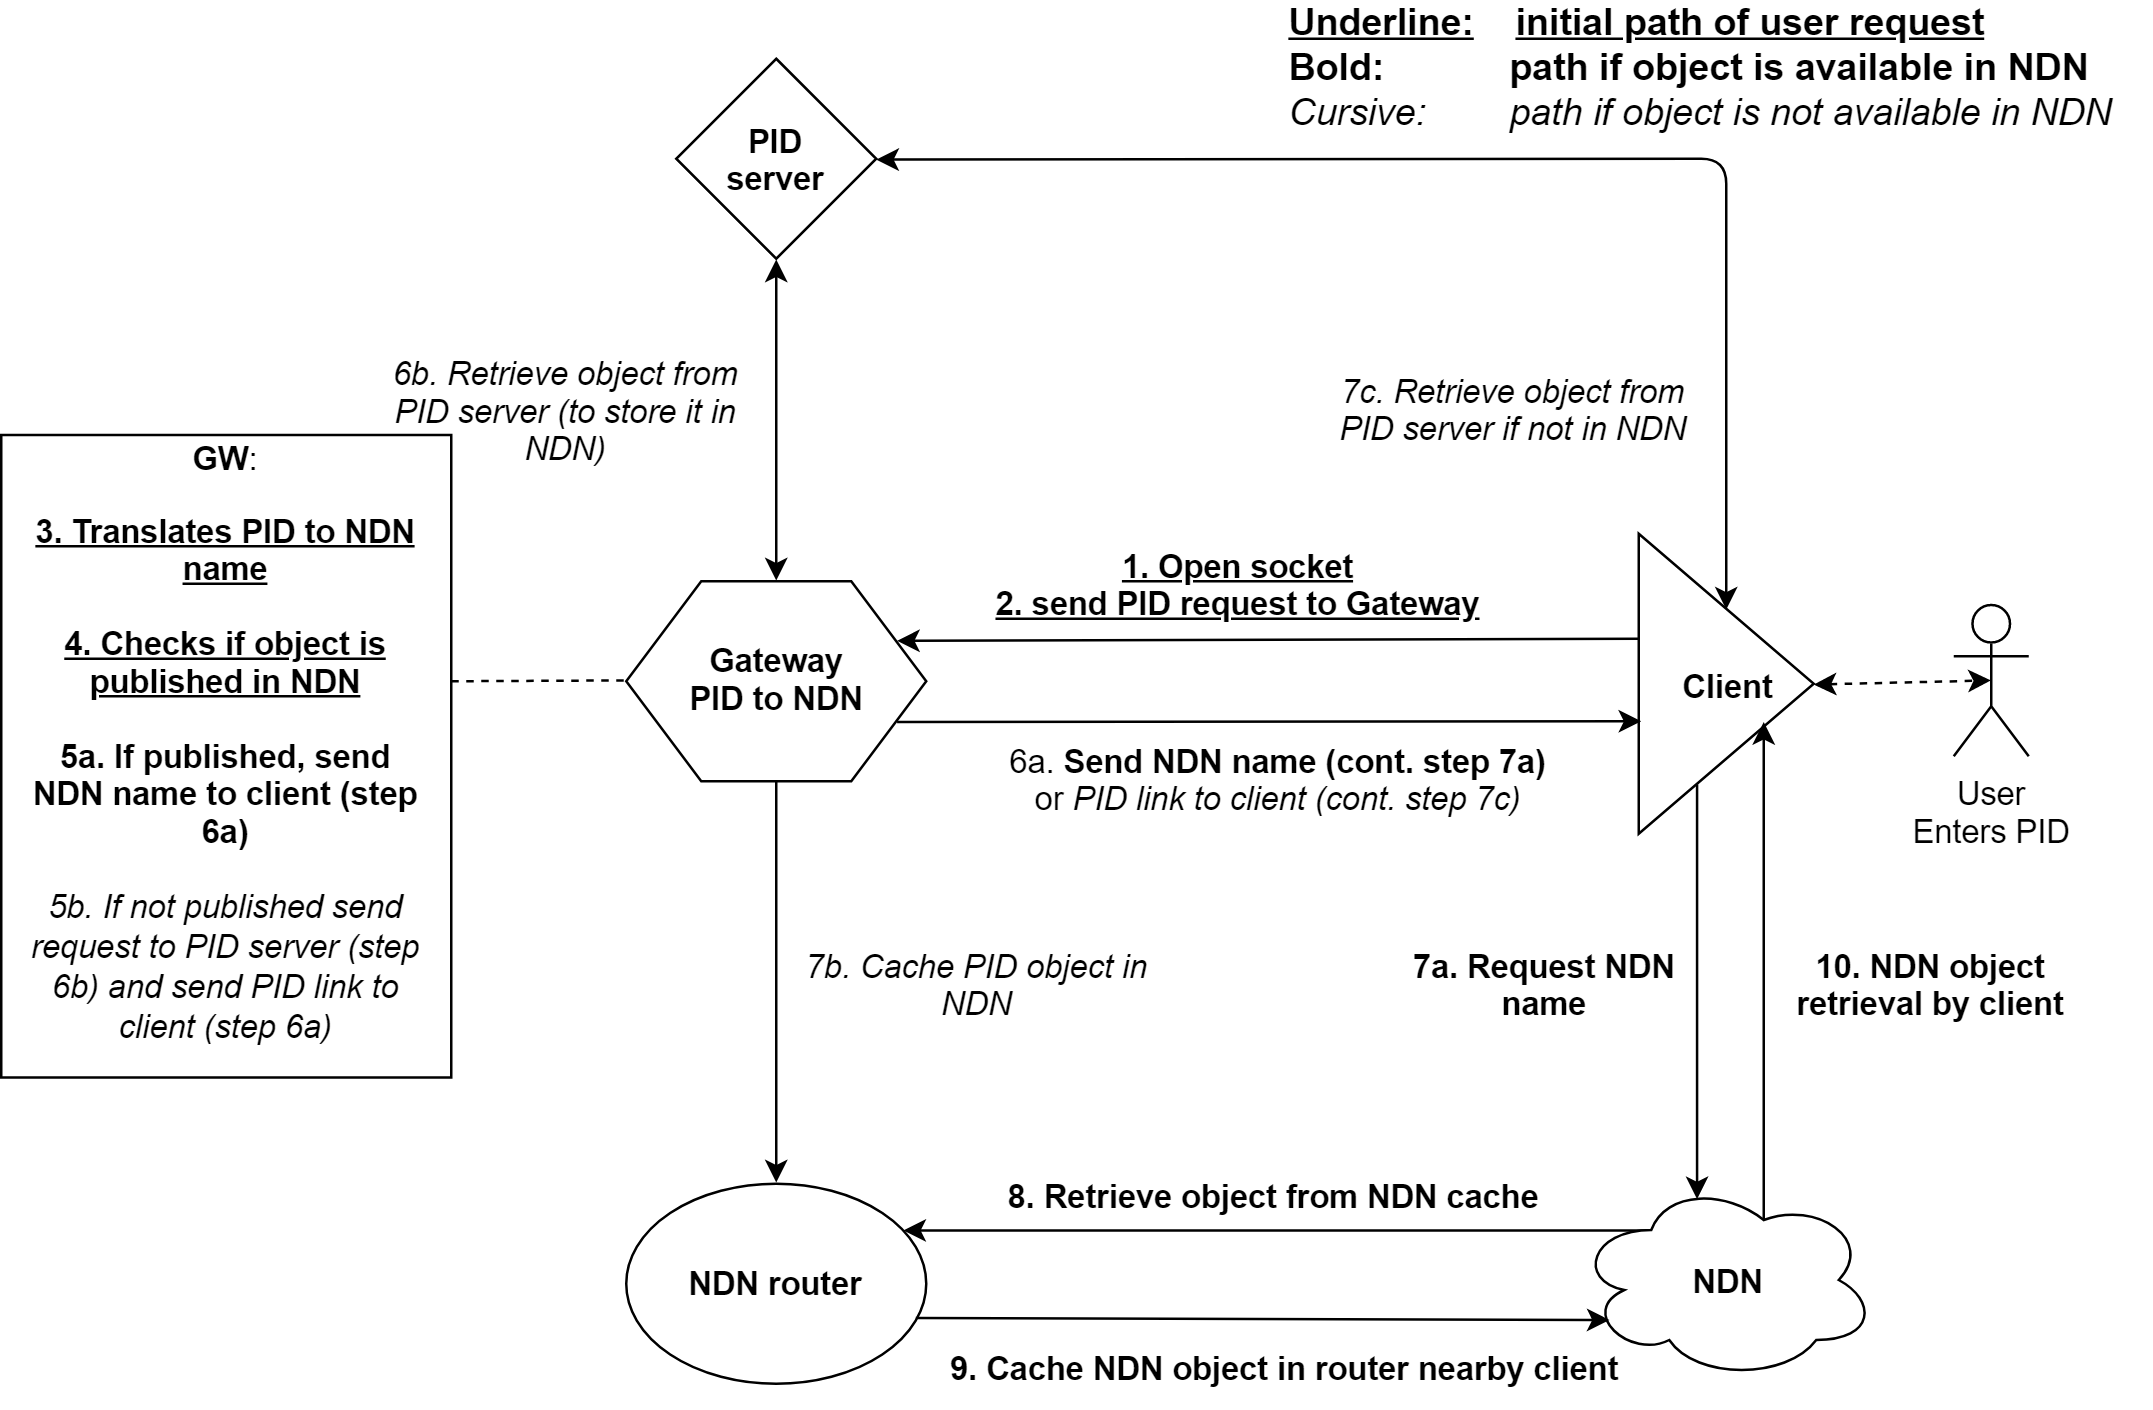
\includegraphics[width=\columnwidth]{images/PIDtoNDN.png}
\caption{\gls{ndn} virtual function based planning for achieving \gls{pid} interoperability}
\label{fig:sdc_model}
\end{figure}
% \end{figure*}

The gateway is responsible for translating a \gls{pid} to \gls{ndn} compatible name and checks if the requested digital object is already published in \gls{ndn}.

Furthermore, the gateway checks if the digital object is already published in \gls{ndn}. If the digital object is available in \gls{ndn}, then the gateway sends the translated \gls{ndn} name back to the client. The client then retrieves the digital object from \gls{ndn}. If the digital object is not available in \gls{ndn}, then the gateway sends back the \gls{pid} link to the client and caches the digital object in \gls{ndn} for future requests.

We implemented the Handle \gls{pid}, the \gls{urn} \gls{pid} type schema of the national library of the Netherlands, as well as the \gls{doi} type schema of PANGAEA. Based on pattern matching of the \gls{pid} type schema\footnote{\url{https://github.com/AquaL1te/rp2/blob/master/Scripts/pid_server.py#L58-L62}}, the gateway detects what kind of \gls{pid} type it has to process. Then, when a \gls{pid} type matches, the associated function is called to translate the \gls{pid} to an \gls{ndn} compatible name\footnote{\url{https://github.com/AquaL1te/rp2/blob/master/Scripts/pid_server.py#L17-L37}}. The matching patterns of most standardized \gls{pid} type schemas are documented in the \gls{epic} \gls{dtr}, and can be implemented in the gateway \cite{dtr} to support a wide range of \gls{pid} types. 


\subsection{NDN on virtual infrastructures}
The \gls{ndn} planning component models the \gls{ndn} function as containers, and plan an \gls{ndn} environment based on the VM based virtual infrastructure. Fig. \ref{fig:high-level-network-design} illustrates the basic idea.

\begin{figure}[H]
\centering
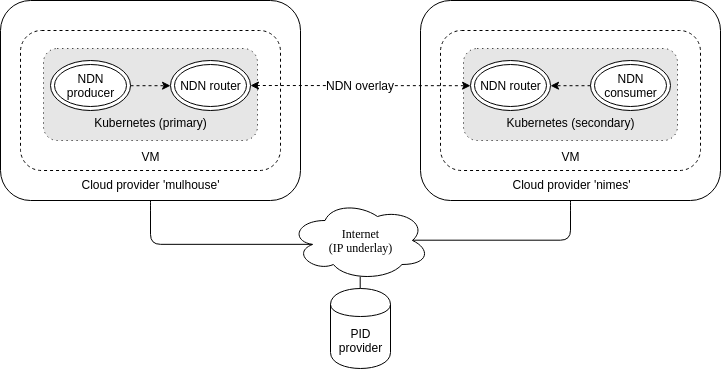
\includegraphics[width=\columnwidth]{images/high-level-network-design.png}
\caption{High-level network design.}
\label{fig:high-level-network-design}
\end{figure}

The planning procedure is designed based on the basic principle in \cite{mccabe2010network}, but in the following steps:
\begin{enumerate}
    \item Select the proper size of the virtual machine, based on the location of the data sources and the users;
    \item Based on the typical size of the data objects, estimate the optimal size of the cache of each node. This has to bounded with the total budget planned for the environment. 
    \item Place the \gls{ndn} function on the nodes e.g., \gls{ndn} gateways, and the \gls{ndn} routing functions. 
\end{enumerate}

A virtual \gls{ndn} environment is thus a set of networked virtual machine, with the deployment of containers for \gls{ndn} functions. The description of the virtual machine, topologies, and the \gls{ndn} functions are described using a standardised language called \gls{tosca} \cite{tosca-standard}.
The \gls{tosca} provides a rich set of elements, e.g., nodes, relationships and interfaces, to describe the basic structure the virtual machines. The relation between virtual machines and the \gls{ndn} functions are described using the relation such as `dependsOn', `hostedOn' and `connectsTo'. 

Interfaces are used to control the life cycle of a component and consist as a set of hooks to trigger actions, these actions are create, configure, start, stop or delete. These hooks can be triggered to e.g. configure and create containers, stop or start a service or do system maintenance such as delete artifacts after a service is stopped. An example is shown in Fig. \ref{fig:tosca-diagram}.
\begin{figure*}[ht]
\centering
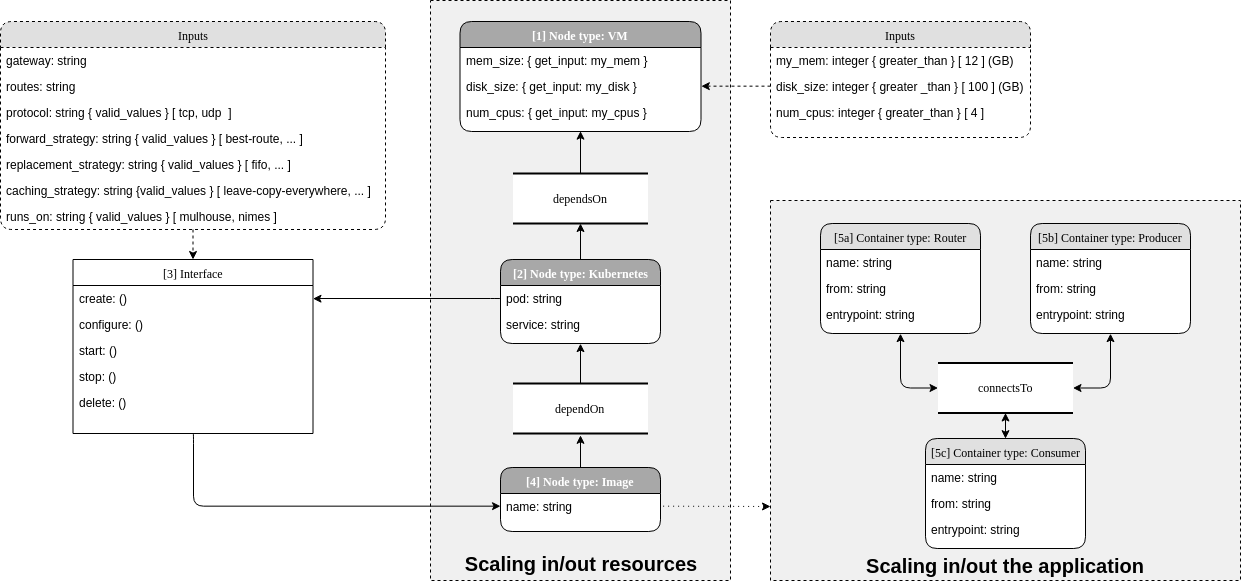
\includegraphics[width=\textwidth]{images/tosca-diagram.png}
\caption{TOSCA diagram.}
\label{fig:tosca-diagram}
\end{figure*}
In Fig. \ref{fig:tosca-diagram}, a \gls{tosca} diagram is illustrated. This diagram represents an abstract template description of the \gls{tosca} relationships, in which the gray rectangular boxes are the core scalability factors. The scaling properties are highlighted in the rectangular areas. The left area, highlighted as `scaling in/out resources' contains a dependency chain of several virtual \gls{ndn} functions. This dependency chain is also depicted numerically.


\subsection{NDN automation}

An \gls{ndn} is typically distributed geographically. Therefore, deploying \gls{ndn} on Cloud providers helps distribution. The heterogeneous nature in Cloud environments can make deployment automation and management complicated. The \gls{ndn4di} automates the provisioning of the \gls{tosca} description in the virtual \gls{ndn} environment using \gls{drip} \cite{koulouzis2019time}, an engine developed by the same team in earlier projects. Kubernetes is employed to automate the orchestration of the containerized \gls{ndn} functions. 

In the example in Fig. \ref{fig:tosca-diagram}, a VM needs to be first provisioned (step 1), before a pod can be deployed on Kubernetes (step 2 to 5). This is described by the `dependsOn' relationship. Furthermore, with the requirements defined, input constraints are described. These constraints are used by the orchestrator to make sure that the \gls{ndn} infrastructure has sufficient resources available to operate. Once a VM is deployed, the dependency for Kubernetes is satisfied, thus Kubernetes can then be setup (step 2). Kubernetes can then deploy pods by the use of interfaces (step 3). These interfaces feed the containers with environment variables such as the gateway, a list of routes, the transport protocol for \gls{ndn}, the \gls{ndn} strategies and on which Kubernetes node this pod should run. The environment variables are given to the interface via the \gls{tosca} inputs. These environment variables are then used by scripts that run inside the pods to setup \gls{ndn}. Several constraints are set for these environment variables such as which valid transport protocols can be used for \gls{ndn}, which \gls{ndn} strategies are valid and which nodes are available. These constraints are defined with e.g. `valid\_values' or `greater\_than' definitions. These constraints help to guide the orchestrator to verify the inputs that are given for the template description. As illustrated in the second gray area `scaling in/out the application', several pods can be instantiated (step 5a, 5b and 5c) from the image (step 4). These pods enable the virtual \gls{ndn} functions. These pods establish the \gls{ndn} and therefore are connected via the `connectsTo' relationship. This network expands over to other Kubernetes nodes in the cluster by the use of the Kubernetes built-in overlay network.

\section{System prototype}
\label{ndn-planning-deployment}
The data publishing tool is prototyped as a service, which provide interface for both user interaction \ref{fig:publishingagent} and RESTful API. Via the interface, a user can configure expected external repository, select data snapshot from the version control system, and perform the publishing operation to obtain a \gls{pid} for it. 
\begin{figure}
\centering
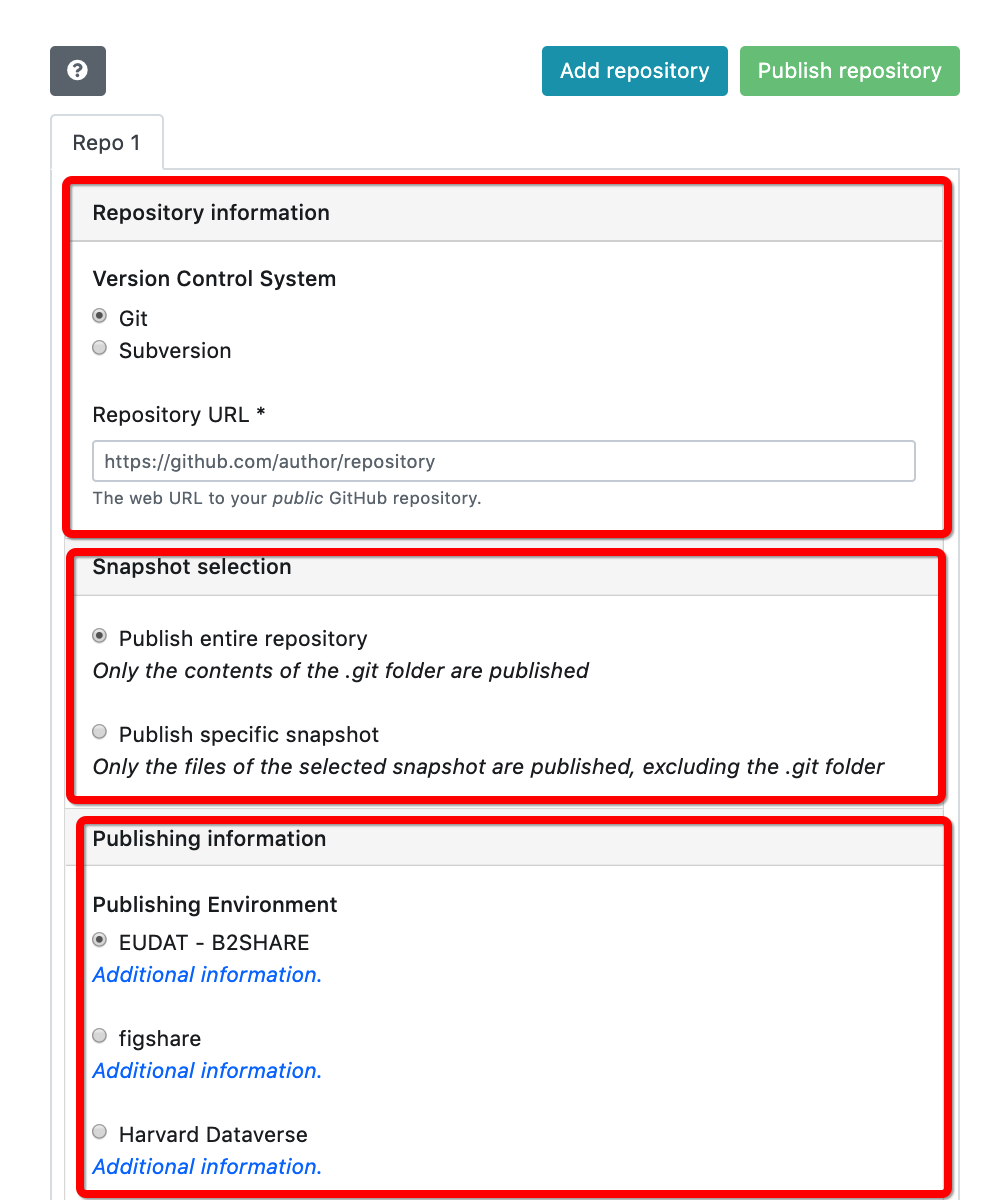
\includegraphics[width=0.4\textwidth]{images/publishingagent.png}
\caption{Screen snapshot of the publishing tool.}
\label{fig:publishingagent}
\end{figure}

In our prototype we implemented the Handle \gls{pid} type within our \gls{pid} server. Furthermore, we also implemented the \gls{urn} \gls{pid} type of the national library of the Netherlands, as well as the \gls{doi} type of PANGAEA. Based on pattern matching of the \gls{pid} type\footnote{\url{https://github.com/AquaL1te/rp2/blob/master/Scripts/pid_server.py#L58-L62}}, the gateway detects what kind of \gls{pid} type it has to process. Then, the associated function in the code is called to translate the \gls{pid} to \gls{ndn} name and appends the corresponding link of the web resolver of the \gls{pid} type it receives\footnote{\url{https://github.com/AquaL1te/rp2/blob/master/Scripts/pid_server.py#L17-L37}}. The patterns of most standardized \gls{pid} types are documented in the \gls{epic} \gls{dtr}\footnote{\url{http://dtr-test.pidconsortium.eu}}.


%  The Ansible playbooks for configuration management and contains a deployment agent for e.g. Kubernetes. 
 

% add sed command to substitute config lines in nfd.conf
The orchestrators mentioned when combined with a \gls{tosca} parser are still in a prototype phase. Therefore, in our prototype we deployed the VMs and Kubernetes nodes manually. In practice the life cycle of also the Kubernetes pods are managed by a \gls{tosca} orchestrator. Without having a \gls{tosca}-ready orchestrator available, steps 2 through 5 in Fig. \ref{fig:tosca-diagram} were be carried out by Kubernetes exclusively. This was done by defining the configuration properties of the pods manually\footnote{\url{https://github.com/AquaL1te/rp2/blob/master/Kubernetes/expanded-cluster.yml}}. These properties include the \gls{ndn} function name, e.g. router, producer or consumer. And also includes the routes (\gls{ndn} prefixes) and the associated \gls{ndn} face with the transport protocol to use (TCP or UDP). These parameters were then inserted into the \gls{ndn} \gls{fib} by the scripts that were executed inside the pod\footnote{\url{https://github.com/AquaL1te/rp2/blob/master/Docker/producer/docker-entrypoint.sh}}. The \gls{ndn} strategies were also configured by these scripts.

%Furthermore, if it is not defined where a pod should be running, Kubernetes will make this decision itself, based on the known resources in the Kubernetes cluster. If for example a Kubernetes node has more memory to spare than other nodes, then Kubernetes will likely decide to spawn the pod there. This Kubernetes node could potentially run in a Cloud provider located in another geographical area. Since the purpose is to provide data distribution through the use of \gls{ndn}, locality becomes a key factor. Therefore, a pod is specifically assigned to a Kubernetes node in order to provide in-network caching in a specific geographical area.

%The methods discussed offer a combined way to plan and deploy a data distribution network. McCabe can be used to methodologically establish the performance requirements. \gls{tosca} can be used to apply these performance requirements to the virtualized environment from a central deployment and management description. For the size of this prototype the McCabe method is extra overhead. However, the prototype is only used to demonstrate the train of thought. The methods discussed can be applied to larger deployments where the McCabe method will be more valuable.

%In conclusion, the \gls{pid} to \gls{ndn} name translation prototype (section \ref{interoperablity}) is integrated as \gls{nfv} pods in our deployment prototype. This enables flexible scaling by the use of Cloud providers.

\subsection{Performance characterstics}
The current prototype of \gls{ndn4di} has been tested in a test environment illustrated in Fig. \ref{fig:high-level-network-design}. We ran the following performance tests within our proof of concept using a 10MB, 100MB, 250MB, 500MB and a 1000MB data digital object size. We performed the performance tests ten times for each digital object size and protocol. The different object sizes were chosen in order to determine if there is a certain trend between the object size and performance. The performance trend is illustrated in Fig. \ref{fig:perftest-6} and shows the average of the test runs. We can observe that \gls{ndn} over UDP outperforms the TCP/IP connection used for retrieving data objects from the Handle \gls{pid} server that we setup with all chosen object sizes. Furthermore, \gls{ndn} over TCP outperforms \gls{ndn} over UDP. This result correlates with the research done by Lim et al. \cite{lim2018ndn}. Fig. \ref{fig:perftest-6} illustrates that the performance converges with a 250MB digital object. We can therefore conclude that the relative performance difference between \gls{ndn} and TCP/IP becomes smaller with object sizes larger than 250MB. Research done by Oran concluded that this observation is due to \gls{ndn}'s nature of handling big object sizes. Which may cause a performance problem due to the cost of retransmission when interests are retransmitted (or re-issued) \cite{ndn-objects}.

\begin{figure}[H]
\centering
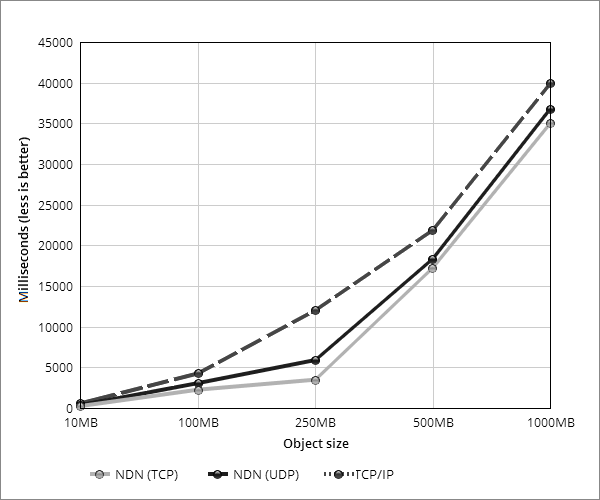
\includegraphics[width=\columnwidth]{images/linechart5.png}
\caption{Object size to performance relation.}
\label{fig:perftest-6}
\end{figure}

The results gathered were merely based on best-effort test scenarios and are inconclusive. Therefore, further and more detailed research is required.

\subsection{a SeaDataNet case study} % title probaly needs to be improved
% * with ndn4di multiple pid types can be used within ndn (in contrast with naas4pid, which has 1 pid type)
% * performance can adjusted to the needs of the users by the use of tosca + nfv
% * data is put closer to the user by the use of in-network caching, reducing latency, but also network load on seadatanet

    % \item Fault tolerance challenges. The SeaDataNet originally only gathers metadata from remote repositories, and the user has to access the individual remote repository to obtain data. Such client-server style not only creates high load for the repository but also network traffic congestion.
    % \item Performance challenges. A Cloud replica has been created in SeaDataNet to duplicate each remote repository in the Cloud. In this way, the clients can directly retrieve the copy of data assets from the Cloud server. However, such solution also needs careful customization for load-balancing and service placement to reach the required quality of service quality or user experiences.
    % \item Scalability challenges. The SeaDataCloud has to face the continuous growth of both data providers and the user communities. In many cases, geo special data retrieval needs calculation of the region, layers and the time duration. The system has to face scalability challenges of both network and the server capacity. 

Taking the data management scenario of SeaDataNet described in \ref{problem-background} as an example, the proposed \gls{ndn4di} solution can be utilised in several ways. 
\begin{enumerate}
    \item Fault tolerance challenges. By using the on demand \gls{ndn} environment, the data objects from the distributed repositories will be cached based on the access frequency in the Cloud. The planner can be used to compute and optimize cache sizes, and the topology of the \gls{ndn} nodes. In this case, the single point failure of the remote repository can be voided.  
    \item Performance and scalability challenges. Using the containerised \gls{ndn} function over virtual infrastructure, nodes and the containers can be scaled out efficiently. We have not demonstrated the software in this paper; however, the feasibility of auto scaling of the virtual machine and the auto configuration of \gls{ndn} nodes can clearly realise it.  
    \item \gls{pid} of data objects. The data publishing tool can be utilised by the remote data sources to automate the publishing of their data products. In the context data infrastructure, \gls{pid} is often not a technical question; the most difficult part is to convenience community to agree on a standard. In this paper, we did not discuss that part, but only focus on the technical aspects in automating the publishing workflow. 
    \item With \gls{ndn4di}, multiple \gls{pid} types can be integrated into the \gls{ndn}. Furthermore, by utilizing \gls{ndn}, network load may be more distributed by the use of in-network caching, which also lowers latency for the data consumers. \gls{ndn4di} allows flexible scaling by the use of \gls{nfv} and Cloud providers. This flexibility mostly stems from the central point of orchestration which enables an infrastructure to adjust for higher network loads.
\end{enumerate}

%With \gls{ndn4di}, multiple \gls{pid} types can be integrated into the \gls{ndn}. Furthermore, by utilizing \gls{ndn}, network load may be more distributed by the use of in-network caching, which also lowers latency for the data consumers. \gls{ndn4di} allows flexible scaling by the use of \gls{nfv} and Cloud providers. This flexibility mostly stems from the central point of orchestration which enables an infrastructure to adjust for higher network loads.


\section{Summary}
In this paper, we discussed the data sharing challenges in the data infrastructures and proposed a \gls{ndn} based solution (\gls{ndn4di}) to tackle the challenge. We presented three key components in the \gls{ndn4di} system, and discussed their prototyps based on the \gls{pid}, Cloud and \gls{ndn} technologies. 

\subsection{Discussion}
%Where traditionally IP is used for host-to-host communication, our prototype utilizes \gls{ndn}. Lim et al. researched and proved the effectiveness of \gls{ndn} for big science workflows. However, the data distribution benefits provided by \gls{ndn} would become unscalable without the means to flexibly maintain the life cycle of such an infrastructure. The prototype we researched and developed offers the means to plan and manage the \gls{ndn} life cycle on a larger scale by utilizing Cloud providers. In contrast, if \gls{ndn} was deployed without the discussed planning and deployment methods, an alternative would then be to have custom non-centrally managed deployments for each Cloud environment. Which may create inconsistent deployments and errors. Although such an non-central approach also realizes a data distribution network by the use of \gls{ndn}, it does not scale as well in terms of deployment and management.

We adopted a system based network planning approach presented by McCabe to do  high-level design of the \gls{ndn} in \gls{tosca} \cite{mccabe2010network}. By using the \gls{tosca} standard, deployments in \gls{tosca}-ready Cloud providers are possible with a uniform deployment description. This flexibility allows the data distribution network to scale easily and make management uncomplicated. However, \gls{tosca}-ready Cloud providers are still rare, for our prototype to be more relevant, a wider adoption is needed.

% Due to the nature of Kubernetes, pods are deployed based on the resource requirements of a pod and the resource availability inside a cluster. Pods that run \gls{ndn} functions are not only interested in Kubernetes resources, but their true value is mainly determined on locality. This is due to the distributed nature of \gls{ndn}, which depends on in-network caching along the network path between data producers and consumers. If Kubernetes does not deploy a pod where \gls{ndn} resources are needed, then human intervention is needed to specify on which Kubernetes node a pod must run. Therefore, if Kubernetes could be extended with the intelligence of also \gls{ndn}'s resource needs, it could deploy pods automatically in a certain geographical area in order to increase cache hits.

The \gls{ndn} configuration is still complex; a generic solution is still lack, which was due to the immature \gls{ndn} routing protocols. However there are two promising routing protocols in development; \gls{ospfn} by Lan Wang et. al. \cite{ndn-ospfn2} and \gls{nlsr} \cite{nlsr}. With a routing protocol, the \gls{ndn} management process would become less complicated and more resilient.

Furthermore, in data infrastructure identification services are used and utilize different \gls{pid} schemas. Our prototype offers a better integration between the identification and the data transmission services. However, our prototype exists outside of the \gls{ndn} source code. For the best application of this functionality, we recommend the integration of these interoperability functionalities into the native \gls{ndn} source code. This would remove the need to run a translation gateway.

Large data infrastructures are in general a federated architecture, where each federation is responsible for its own budget and infrastructure. However, our prototype assumes central control over the \gls{ndn}. Our prototype could be approached in several ways. The discussed solutions could be deployed as an internal data-sharing platform per infrastructure and interconnect those \glspl{ndn}, thus maintaining the federated model. Or, it could be deployed as a third party data-sharing platform, where one can deploy and operate the \gls{ndn} for multiple infrastructures. Our research did not explore these subjects. However, it provides the flexibility to deploy these solutions in such a manner.
\subsection{Conclusions}
From the work, we can conclude that cloud environments provide elastic resources for planning and customizing \gls{ndn} based environment for the distributed data infrastructures to share data objects. The automated planning, provisioning and deployment of \gls{ndn} environment is an important to improve the usability of \gls{ndn} in distributed data infrastructures. The proposed \gls{ndn4di} is towards that direction. 

\subsection{Future work}
The work will be continued with case studies with real operational data infrastructures. First, a detailed performance comparison with the current Cloud replica solution used by SeaDataNet and the \gls{ndn4di} will be performed. Moreover, the ENVRI-FAIR is data infrastructure project just started, more than 10 different infrastructures are in the project. In this context, more use cases will be identified to improve the implementation of \gls{ndn4di}.  


\section*{Acknowledgment}
This paper is largely based on the work done by Kees de Jong, MSc (SURFsara) and Anas Younis, MSc \cite{de2019planning}. This research is also supported by the European Union’s Horizon 2020 research and innovation program under Grants No. 824068 (ENVRI-FAIR) and No. 825134 (ARTICONF). 
% how to acknoledge cas? his poster is not published (google scholar)

% \section*{References}
\newacronym{pid}{PID}{Persistent Identifier}
\newacronym{eosc}{EOSC}{European Open Science Cloud}
\newacronym{ndn}{NDN}{Named Data Networking}
\newacronym{icn}{ICN}{Information Centric Networking}
\newacronym{cmmap}{CMMAP}{Center for Multiscale Modeling of Atmospheric Processes}
\newacronym{cmip}{CMIP5}{Coupled Model Intercomparison Project}
\newacronym{uri}{URI}{Uniform Resource Identifier}
\newacronym{url}{URL}{Uniform Resource Locator}
\newacronym{urn}{URN}{Uniform Resource Name}
\newacronym{doi}{DOI}{Digital Object Identifier}
\newacronym{purl}{PURL}{Persistent Uniform Resource Locator}
\newacronym{ark}{ARK}{Archival Resource Key}
\newacronym{tosca}{TOSCA}{Topology and Orchestration Specification for Cloud Applications}
\newacronym{drip}{DRIP}{Dynamic Real-time Infrastructure Planner}
\newacronym{cnri}{CNRI}{Corporation for National Research Initiatives}
\newacronym{fib}{FIB}{Forwarding Information Base}
\newacronym{pit}{PIT}{Pending Interest Table}
\newacronym{cs}{CS}{Content Store}
\newacronym{n2t}{N2T}{Names to Things}
\newacronym{ospfn}{OSPFN}{Open Shortest Path First for NDN}
\newacronym{ghr}{GHR}{Global Handle Registry}
\newacronym{ghs}{GHS}{Global Handle System}
\newacronym{dtr}{DTR}{Data Type Registry}
\newacronym{ra}{RA}{Registration Authority}
\newacronym{idf}{IDF}{International DOI Foundation}
\newacronym{nlsr}{NLSR}{Named-data Link State Routing}
\newacronym{cs3}{CS3}{Cloud Storage Synchronization and Sharing Services}
\newacronym{cdn}{CDN}{Content Delivery Network}
\newacronym{nfv}{NFV}{Network Functions Virtualization}
\newacronym{isbn}{ISBN}{International Standard Book Number}
\newacronym{gpl}{GPLv3}{General Public License}
\newacronym{ddos}{DDoS}{Distributed Denial of Service}
\newacronym{naas4pid}{NaaS4PID}{NDN-as-a-service for PID data objects}
\newacronym{cxx}{NDN-CXX}{NDN C++ library with eXperimental eXtensions}
\newacronym{ccnx}{CCNx}{Content-Centric Networking}
\newacronym{rfc}{RFC}{Request for Comments}
\newacronym{dona}{DONA}{Digital Object Numbering Authority}
\newacronym{ucs}{UCS}{Universal Coded Character Set}
\newacronym{rdf}{RDF}{Resource Description Framework}
\newacronym{oasis}{OASIS}{Organization for the Advancement of Structured Information Standards}
\newacronym{egi}{EGI}{European Grid Infrastructure}
\newacronym{exogeni}{ExoGENI}{Exo Global Environment for Network Innovation}
\newacronym{fp7}{EU FP7}{European Seventh Framework Programme}
\newacronym{do}{DO}{Digital Object}
\newacronym{dcx}{DCX}{Dublin Core}
\newacronym{anp}{ANP}{Algemeen Nederlands Persbureau}
\newacronym{nr}{NR}{National Resolver}
\newacronym{ir}{IR}{Institutional Repository}
\newacronym{doip}{DOIP}{Digital Object Interface Protocol}
\newacronym{fairness}{FAIRness}{Findability, Accessibility, Interoperability and Re-usability}
\newacronym{icos}{ICOS}{Integrated Carbon Observation System Research Infrastructure}
\newacronym{ri}{RI}{Research Infrastructure}
\newacronym{actris}{ACTRIS}{Aerosol, Clouds and Trace Gases}
\newacronym{epos}{EPOS}{European Plate Observing System}
\newacronym{envri}{ENVRI-FAIR}{ENVironmental Research Infrastructures building Fair services Accessible for society, Innovation and Research}
\newacronym{rda}{RDA}{Research Data Alliance}
\newacronym{sdn}{SDN}{Software Defined Networking}
\newacronym{ndn4di}{NDN4DI}{Named Data Networking for Data Infrastructures}
\newacronym{epic}{ePIC}{European Persistent Identifier Consortium}
\newacronym{doa}{DOA}{Digital Object Architecture}

\bibliographystyle{./bibliography/IEEEtran}
\bibliography{./bibliography/IEEEabrv,./bibliography/IEEEexample}

\end{document}